\documentclass{article}
\usepackage{mathtools}
\usepackage[margin=1in]{geometry}
\usepackage[doublespacing]{setspace}
\usepackage{enumitem}
\usepackage{cite}
\usepackage{graphicx}
\graphicspath{ {images/} }

\begin{document}
    \begin{center}
        \bf{\large Physics 182 \\ Thesis Introduction Rough Draft V2 \\ Christopher Milke}
    \end{center}


    \vspace{10mm}
    \begin{center}
        \underline{ \large An Introduction to the International Linear Collider }
    \end{center}
        \begin{center} \bf{What is the ILC and Why Does it Need to Exist?} \end{center}

        \begin{figure}[h] 
            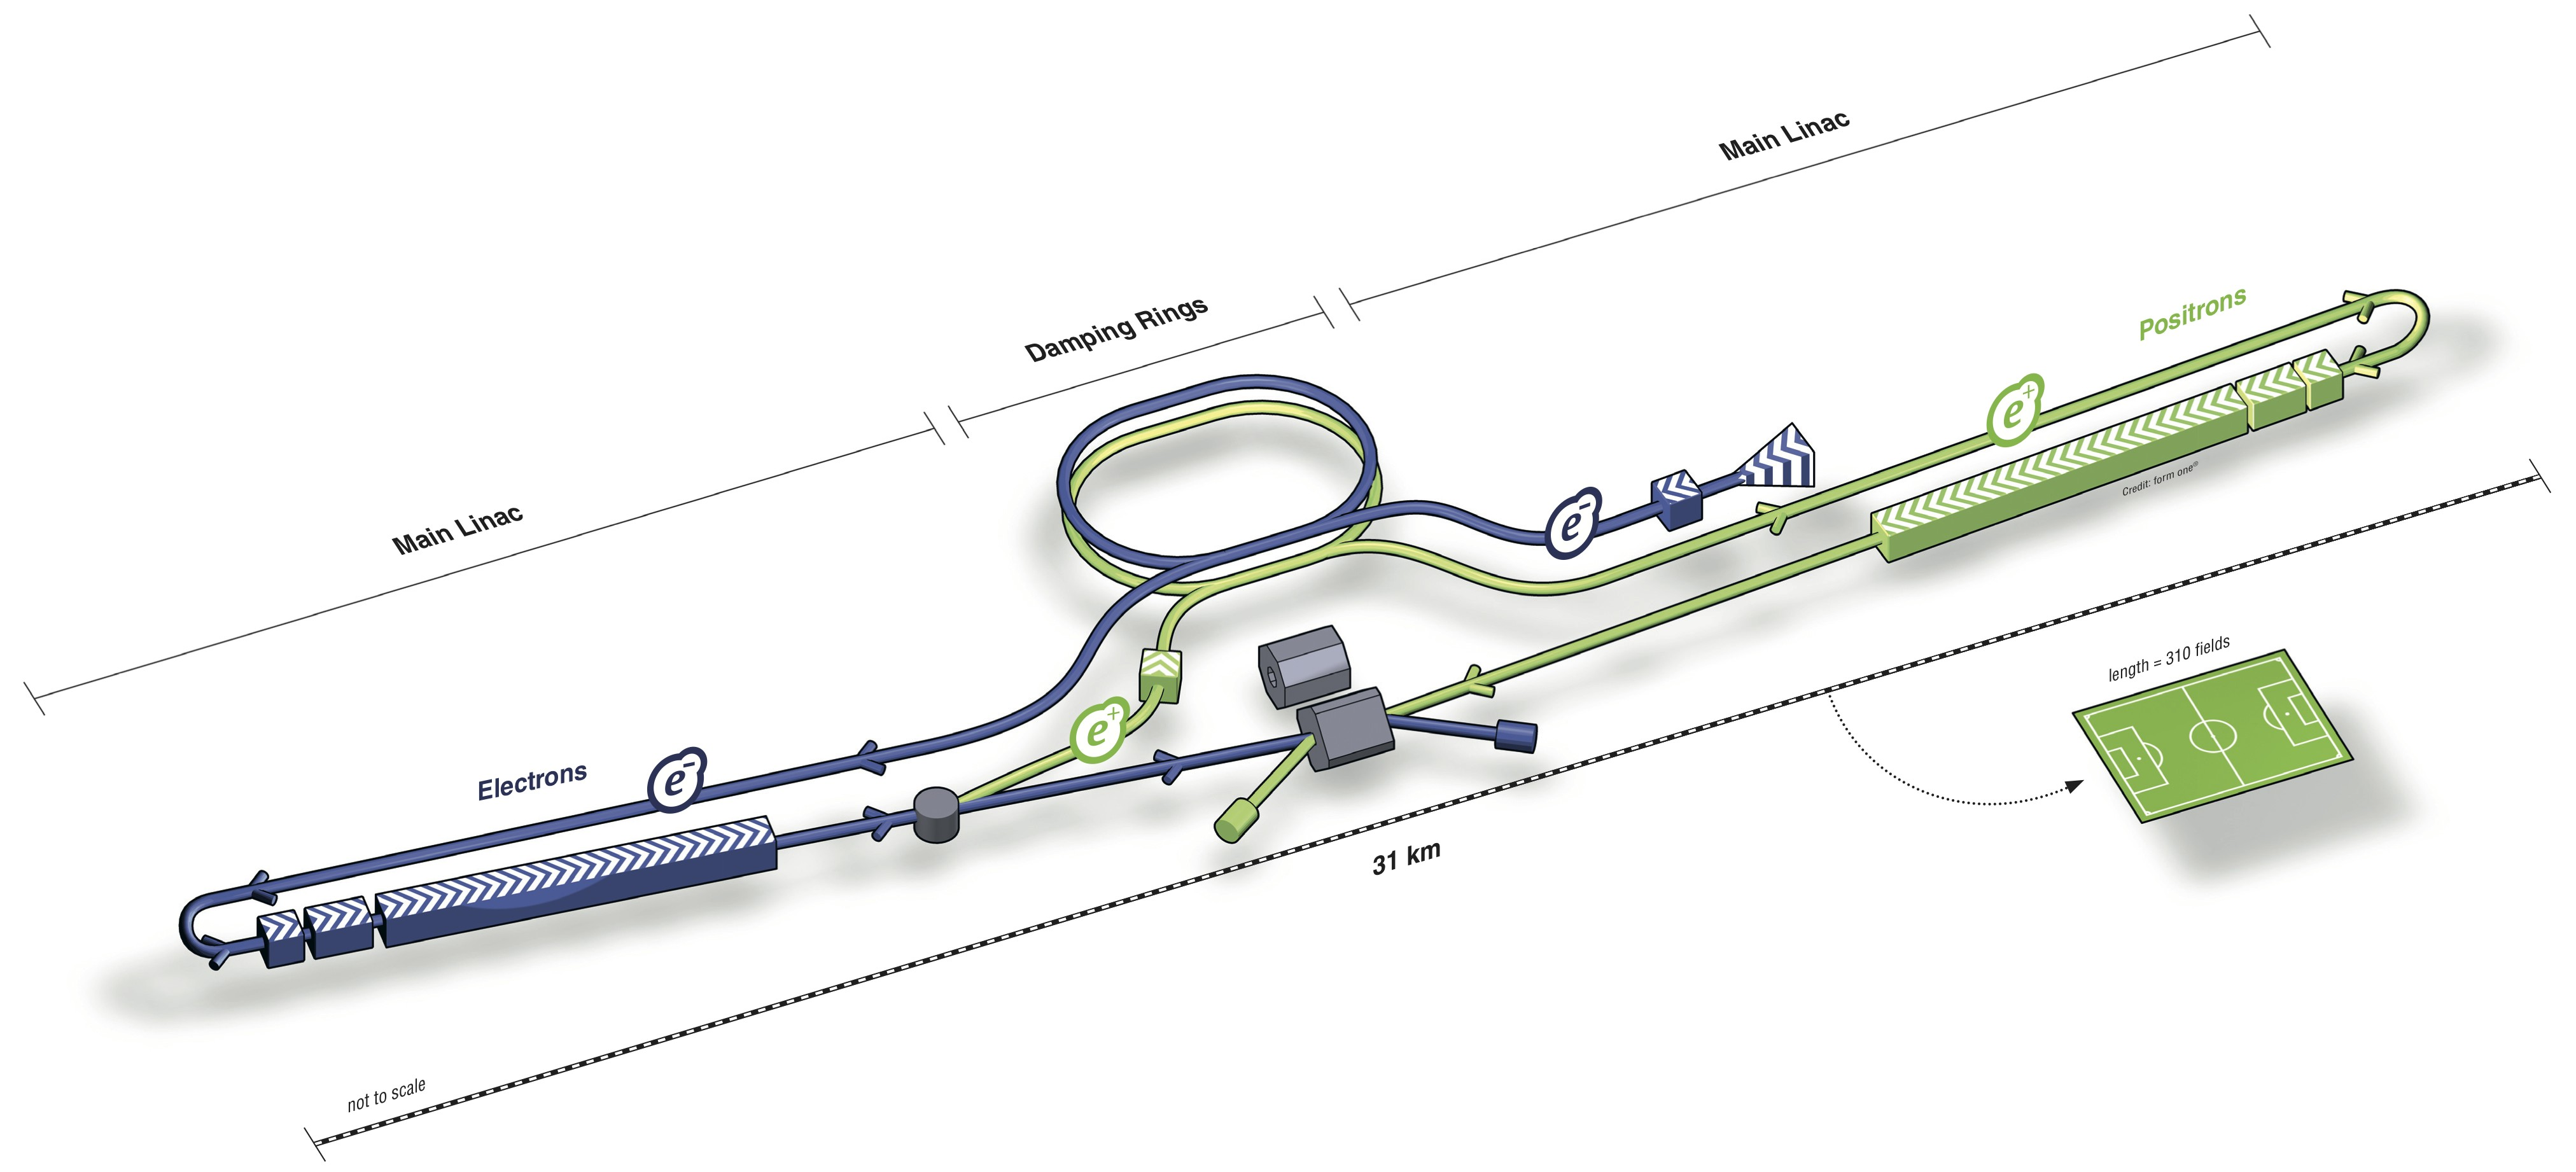
\includegraphics[width=\textwidth]{ilcoverview}
            \centering
            \caption{Overview of the ILC}
            \label{ilcoverview}
        \end{figure}

        The International Linear Collider (ILC) is a 30 kilometer long \cite{parton} linear particle accelerator \cite{specs} which will collide electrons and positrons together at 500 GeV energies. It will primarily be used for studying the properties of the Higgs Boson, attempting to find new dimensions, and trying to discover Supersymetric (SUSY) particles. All three of these are already being pursued by the much more powerful Large Hadron Collider (LHC), which begs the question of why the ILC is needed. The answer is that, while the LHC is significantly more powerful, the ILC will be significantly more precise. This is because the LHC is, as the name would imply, a hadron collider. In the simplest case, the LHC performs proton-proton collisions. However, protons are not elementary particles. They consist of three quarks and any number of gluons holding those quarks together. A collision between two protons then is actually a collision between six quarks and several gluons. This is a problem for physics studies in particle accelerators, because of something known as a parton distribution function. To understand why, a brief explanation of how one conducts particle accelerator physics studies is in order.

        All the physics processes mentioned, and indeed most other physics processes studied in particle colliders, are studied by reconstructing the paths and energies of particles as they traverse the various detector elements surrounding the particle collision point. The reconstructed paths are then compared to the initial state of the particles that went into the collision. The key statement here is that the comparison is to the particles' \textit{initial} state. While the positions and energies of the protons that are colliding may be well known, the same cannot be said for the individual quarks and gluons the proton is made up of. All that can be done for the constituent particles is to make estimates on where they \textit{might} be based a probabilistic distribution, known as a Parton Distribution Function (PDF). As a result, almost all studies done at the LHC (or any other hadron collider for that matter) face a constant source of significant systematic error on all results it produces. The ILC eliminates this issue entirely by colliding only electrons and positrons, both elementary particles that have no need of PDFs. As a result, the ILC can perform physics studies at a much more precise level, providing details on physics that the LHC cannot.

        \vspace{5mm}
        \begin{center} \bf{An Overview of the Vertex Detector and BeamCal} \end{center}

        %\begin{figure}[h] 
        %    \includegraphics[width=15cm]{sid}
        %    \centering
        %    \caption{View of the Sid}
        %    \label{sid}
        %\end{figure}

        \begin{figure}[h] 
            \includegraphics[width=\textwidth]{sid_zoom1}
            \centering
            \caption{Zoomed in view of the SiD.
                The Vertex Detector is circled in red,
                the BeamCals in magenta.}
            \label{sid_zoom1}
        \end{figure}

        At the crossing of the positron and electron beams is the ILC's interaction point (IP). At any given time the IP can be surrounded by one of two exchangeable detectors: the Large International Detector (ILD) or the Silicon Detector (SiD). The focus in this study will be on the latter of the two. The SiD is an array of trackers and calorimeters over 12 meters long and over 16 meters in diameter. Of the numerous detectors it consists of, the two relevant to this study are the Vertex Detector and Beam Calorimeter (BeamCal). Both detectors are located extremely close to the IP of the SiD, in an area known as the Interaction Region (IR). 
        
        \begin{figure}[h]
            \centering
            \begin{minipage}{0.4\textwidth}
                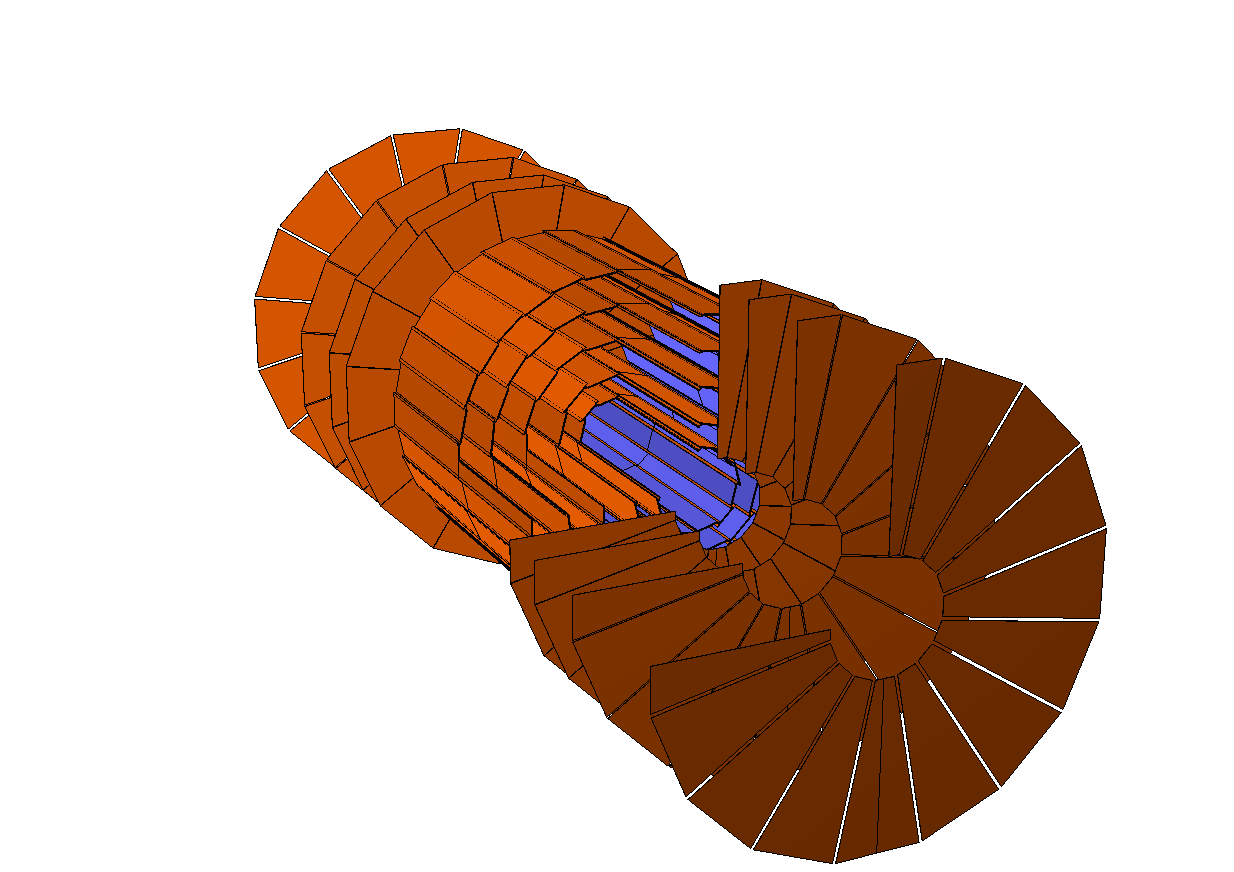
\includegraphics[width=\textwidth]{vertex}
                \caption{Vertex Detector}
                \label{vertex}
            \end{minipage}
            \begin{minipage}{0.4\textwidth}
                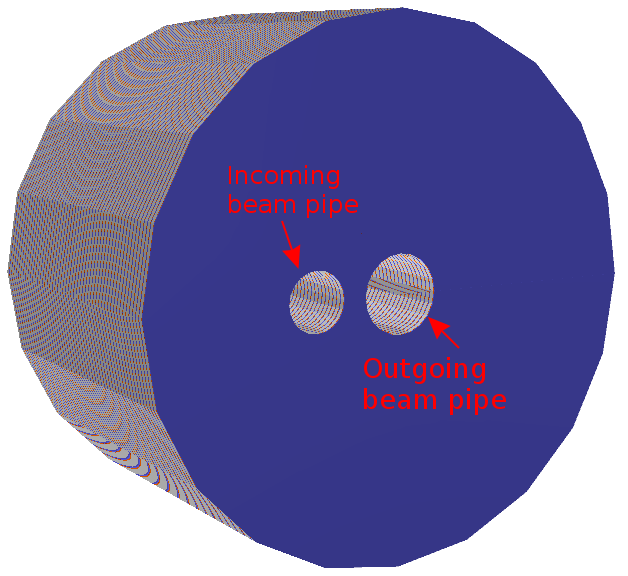
\includegraphics[width=\textwidth]{beamcal_full}
                \caption{Beam Calorimeter}
                \label{beamcal}
            \end{minipage}
        \end{figure}
        
        The Vertex Detector, with a radius of only 6.3 centimeters and a length of 5.2 centimeters, immediately surrounds the IP. The BeamCal (or rather BeamCals, as the entire SiD is mirrored) is a fair distance away from the IP, at 32.65 meters. But with a radius of 14 centimeters, it closely hugs both the incoming and outgoing beam pipes, visible as holes in figure \ref{beamcal}. The locations of the detectors provide unique advantages to each. For the Vertex Detector, surrounding the IP so closely means that it is often the first to detect particles, and is able to detect them before the solenoid's magnetic field has had much chance to deflect them. The BeamCal meanwhile sits in such a far away location, with such a small radius, that the only particles which hit it are those with extremely low transverse momenta. Generally the only particles with such a low trajectory angle are those which have had minimal interaction with other particles, and have thus retained most of their energy. As a result, the BeamCal is hit by some of the highest energy particles produced by the electron/positron collision. Besides their locations though, the Vertex Detector and BeamCal function in almost diametrically opposed ways.

        The Vertex Detector is a tracker-style detector, designed to track the positions of particles as they move through its layers. By identifying hits from a particle across the Vertex Detector's layers, the particle's trajectory can be determined. The Vertex Detector is built to interact with the particle as little as possible, so as not to interfere with the particle's trajectory. Moreover, it is critically important that the occupancy (the number of particles hitting the detector) be kept as low as possible. If the occupancy is too high, then it becomes difficult or impossible to effectively reconstruct particle trajectories. The BeamCal, on the other hand, is designed primarily for calorimetry, determining the energy a particle holds (though it does some position tracking as well). This is accomplished by interspersing silicon detector plates with large amounts of tungsten. The tungsten scatters and absorbs the energy of any particles hitting it, eventually stopping them completely. Energy is then measured by looking at how many layers of tungsten a particle was able to traverse before being stopped. This method of measuring energy is also the basis of a conflict between the Vertex Detector and BeamCal. Because the BeamCal effectively acts as a wall to all incoming particles, some of the particles actually ricochet backwards off of it, in an effect called \textit{albedo}. These showers of albedo particles rebounding off the BeamCal then proceed to fly back towards the IP, and into the Vertex Detector.
        
        The effect requires a careful balancing act. On one end of the scale, albedo increases the occupancy in the Vertex Detector, and should thus be kept to a minimum. On the other end, the BeamCal is a crucial component of the SiD, necessary for low PT (low transverse momentum) particle tagging and beam parameter checking. The BeamCal cannot be removed, but its presence negatively effects the performance of the Vertex Detector. This study aims to research the effects of three independent changes to the architecture of the Interaction Region on this balance, analyzing how each of the changes alters the effectiveness of the Vertex Detector and BeamCal. The first change is with regard to the proximity of the BeamCal to the IP, the second studies the effects of cutting out part of the BeamCal, and the third determines the usefulness of a specialized magnetic field known as the anti-DiD.


    \vspace{10mm}
    \begin{center}
        \underline{\bf{\large Modifications to the SiD}}
    \end{center}
        \begin{center}
            \bf{L Star}
        \end{center}

        The L* of the SiD is a term which refers to the distance between the Interaction Point and the beginning of the cryostat. The most recent technical design report for the SiD specified that for a number of reasons the cryostat needed to be be moved farther away from the Interaction Point, from 3.5 meters to 4.1 meters. The relevance of this change to detector studies is that the BeamCal is attached to the cryostat, so moving the cryostat also means moving the BeamCal (from 2.95 meters to 3.265 meters). This decision has already been made, and so the studies in the analysis section are only to see what the effect of this change is; the results of this study will not affect the design decision.


        \begin{center}
            \bf{Plug Region}
        \end{center}

        \begin{figure}[h]
            \centering
            \begin{minipage}{0.3\textwidth}
                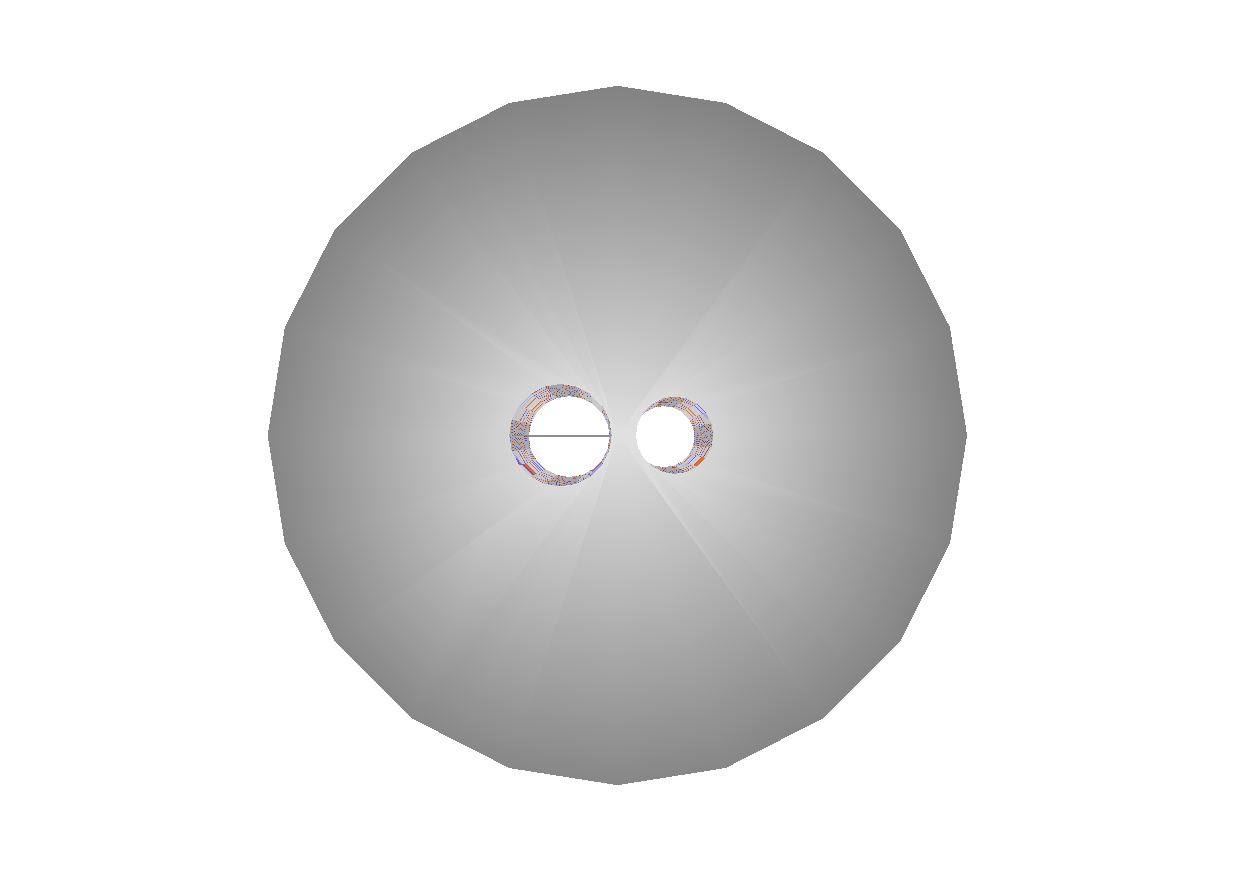
\includegraphics[width=\textwidth]{beamcal_plug}
                \caption{Full plug region}
                \label{beamcal_plug}
            \end{minipage}
            \begin{minipage}{0.3\textwidth}
                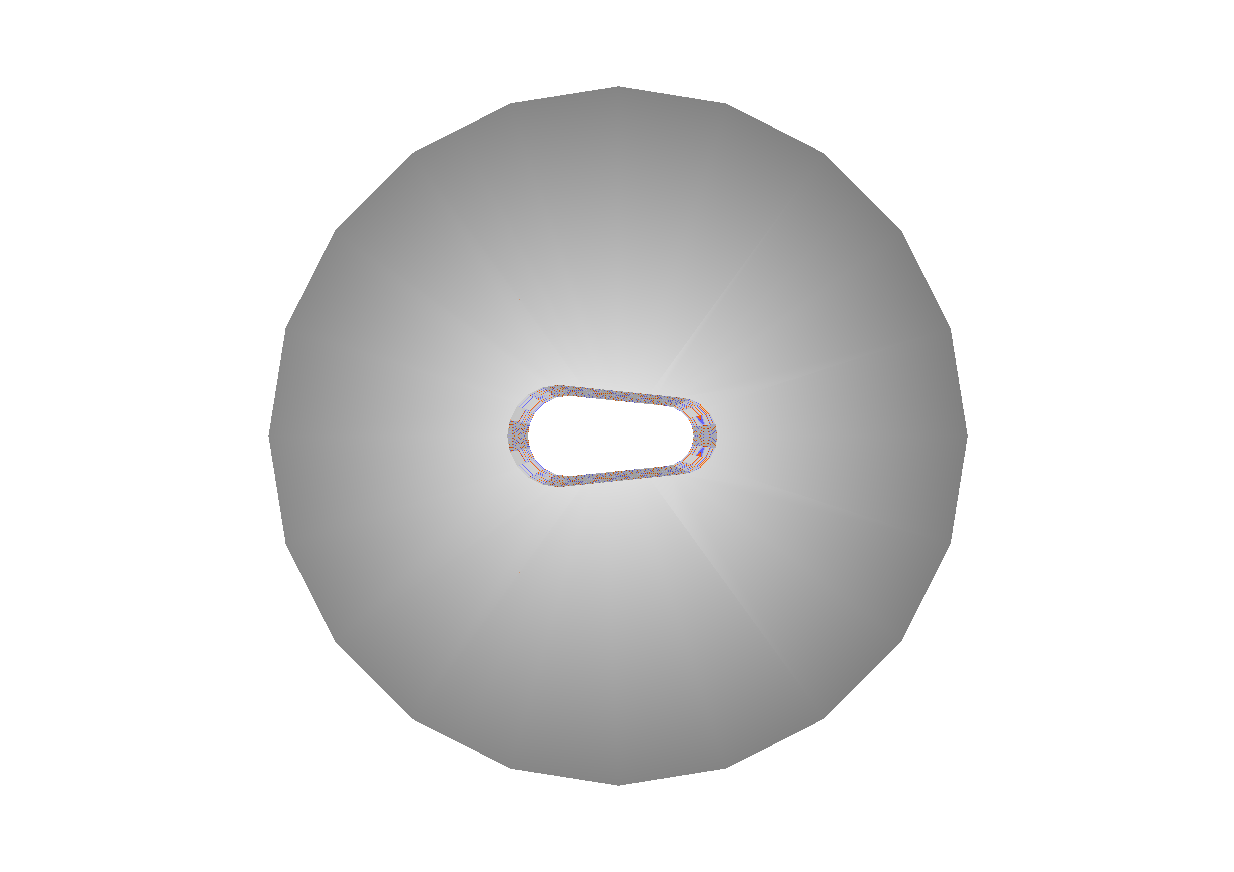
\includegraphics[width=\textwidth]{beamcal_wedge}
                \caption{Wedge cutout}
                \label{beamcal_wedge}
            \end{minipage}
            \begin{minipage}{0.3\textwidth}
                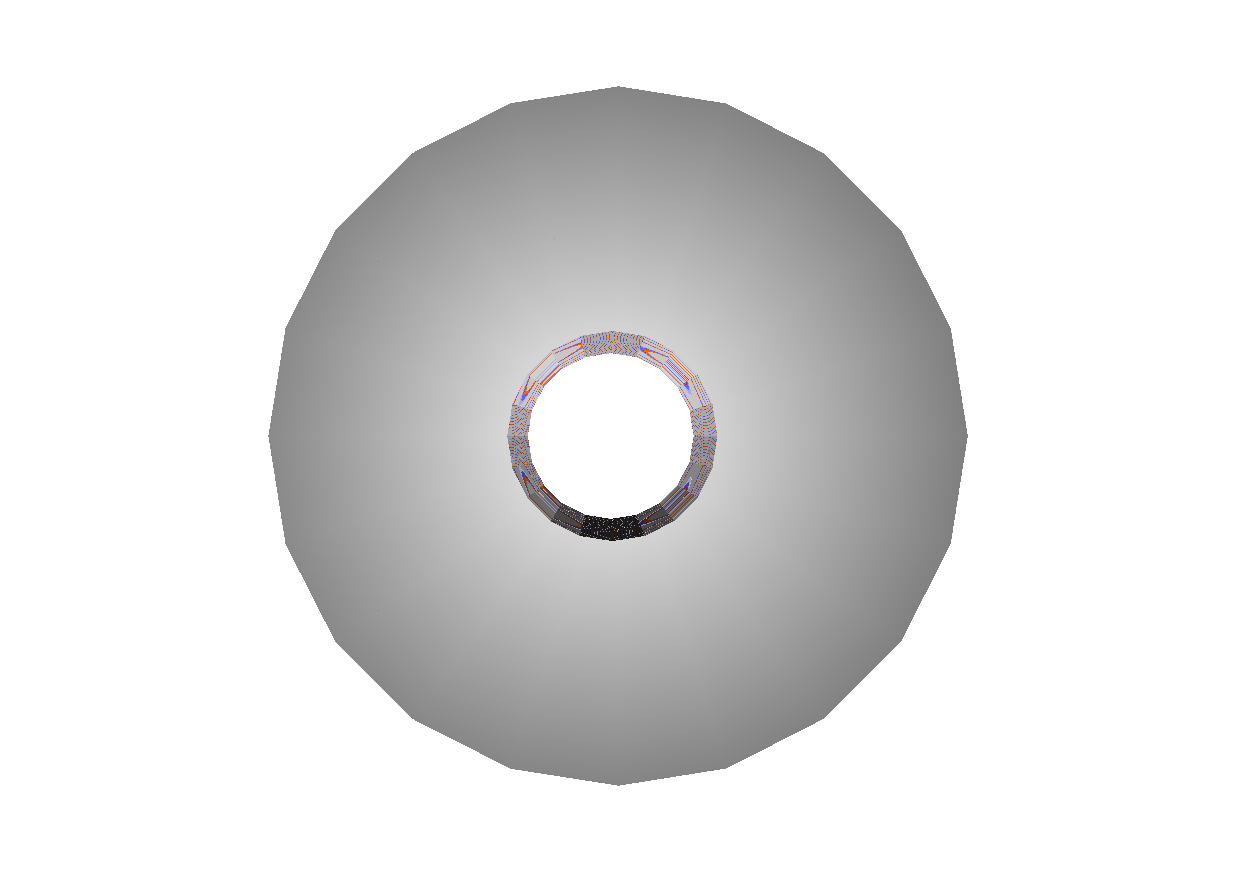
\includegraphics[width=\textwidth]{beamcal_circle}
                \caption{Circle cutout}
                \label{beamcal_circle}
            \end{minipage}
        \end{figure}

        As discussed previously, the BeamCal is hit with a very large amount of energy. The overwhelming majority of the energy is deposited in the central area of the BeamCal, between the two beam pipes. This central location is referred to as the plug region. Removing all or part of the plug region thus has the potential to reduce the energy incident on the face of the BeamCal, and consequently reduce the albedo effect into the Vertex Detector. There are three proposed designs for the plug region (shown in figures \ref{beamcal_plug}, \ref{beamcal_wedge}, and \ref{beamcal_circle}) which remove progressively more detector material. In theory, these designs should provide lower occupancy in the vertex detector, but the cost to the BeamCal is not yet known.


        \begin{center}
            \bf{Anti-Did Magnetic Field}
        \end{center}

        In response to the problem of albedo from the BeamCal into the Vertex Detector, an engineering team proposed the use of a magnetic field known as the DiD, as well as its counterpart, the anti-DiD. The idea of the anti-Did is to redirect low-energy background particles such that they are funneled into the outgoing beampipe of the BeamCal. By redirecting these particles, the particles hitting the BeamCal are reduced, which reduces the albedo into the Vertex Detector. However, the anti-DiD field is very expensive, and has the potential to cause a number of problems with physics analysis. Additionally, a study performed by Thomas Markiewicz \cite{anti-did} suggested that the anti-DiD field could actually be increasing energy deposition outside of the plug region, only causing improvement in a limited area of the detector. For these reasons, a detailed study of the effects of the anti-DiD field on the BeamCal and Vertex Detector is necessary.


        \begin{center}
            \bf{Goals of the Study}
        \end{center}

        The objective of this study will be to update the Interaction Region of the SiD to the most modern and up-to-date specifications, directly using the designs of the SiD's top engineer \cite{excel}. Following from this, the three aforementioned changes will be implemented one at a time, analyzing the effects on the performance of the Vertex Detector and Beam Calorimeter. 


    \bibliography{ref.bib}    
    \bibliographystyle{apalike}


\end{document}
